\documentclass[12pt]{standalone}
\usepackage[utf8]{inputenc}
\usepackage[T1]{fontenc}
\usepackage{times}
\usepackage{amsmath,amssymb}
\usepackage[dvipsnames,svgnames]{xcolor}
\usepackage{tikz}
\usetikzlibrary{decorations.pathreplacing, calc, positioning, shapes.geometric, shapes.symbols, arrows.meta, backgrounds, fit, shapes.misc}
\definecolor{RED}{rgb}{1,0,0}
\definecolor{dmrsfill}{HTML}{CDE2FB}
\definecolor{winblue}{HTML}{0D366B}
\definecolor{inksec}{HTML}{52514E}
\begin{document}
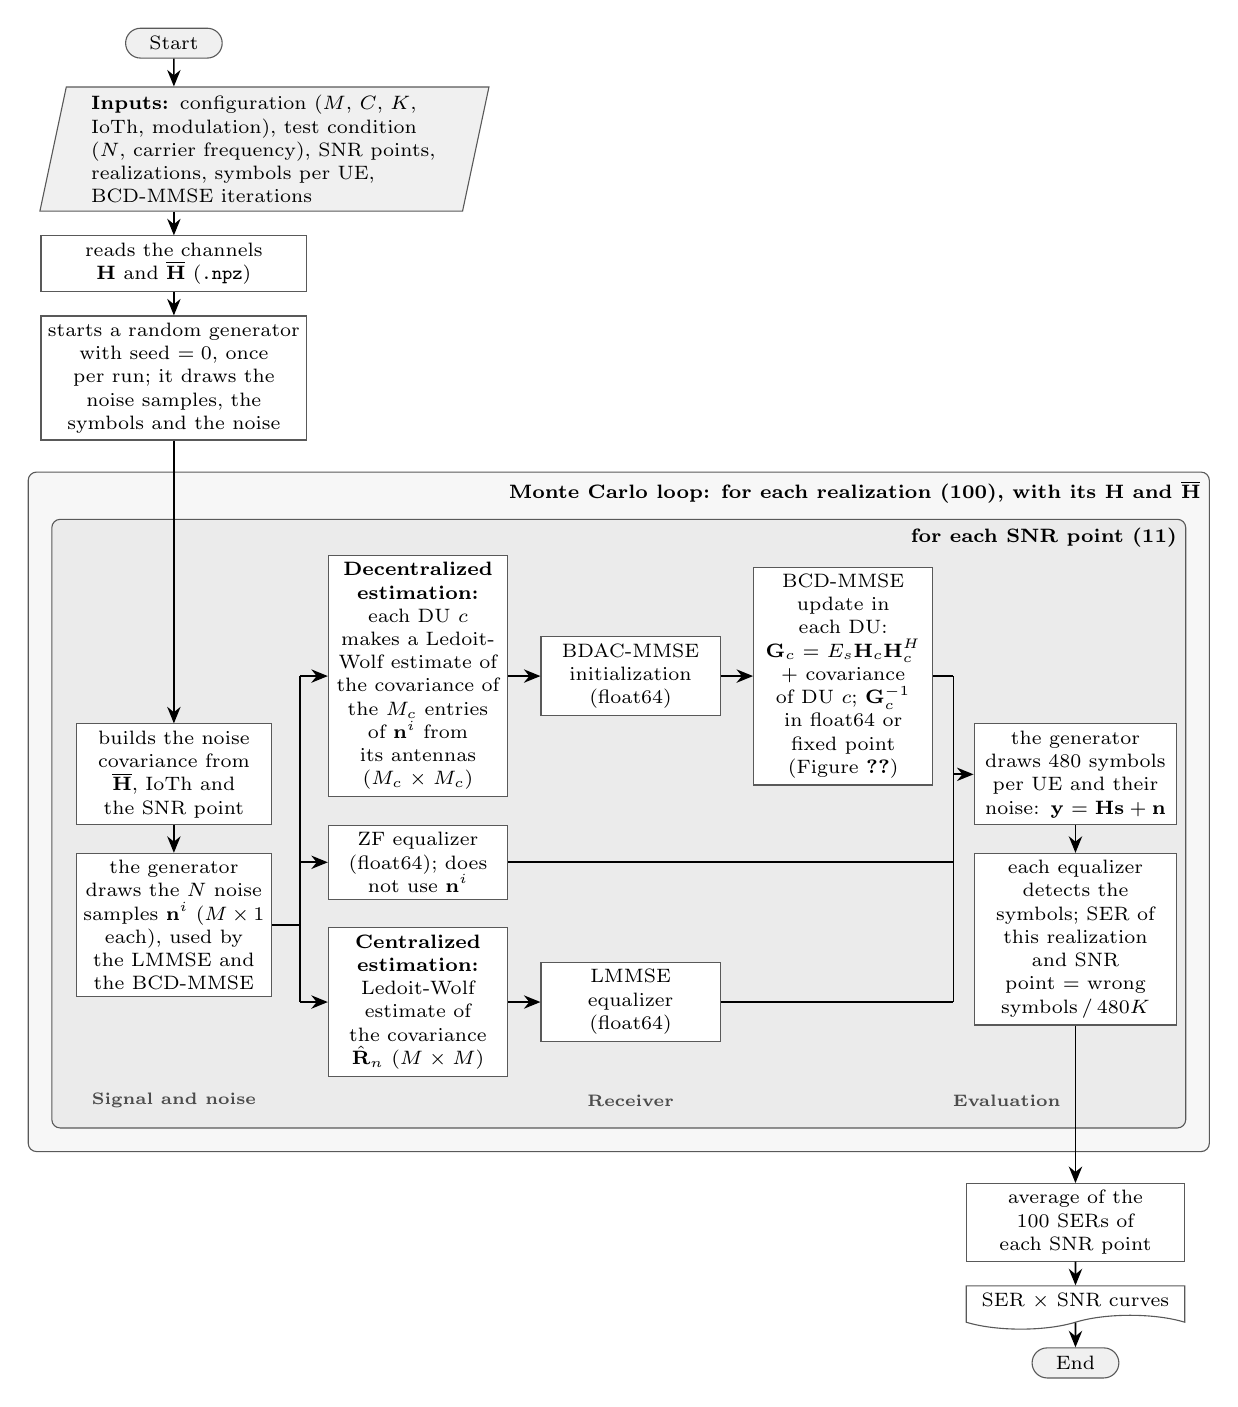
\begin{tikzpicture}[
  font=\fontsize{7}{8.4}\selectfont,
  >={Stealth[length=2.1mm, width=1.7mm]},
  node distance=2.4mm,
  box/.style={draw=black!65, fill=white, align=center,
              inner sep=2.5pt, text width=#1,
              execute at begin node={\hyphenpenalty=10000}},
  box/.default=4.9cm,
  inp/.style={trapezium, trapezium left angle=78, trapezium right angle=102,
              trapezium stretches body, draw=black!65, fill=black!6,
              align=left, inner xsep=9pt, inner ysep=3pt},
  arq/.style={tape, tape bend top=none, draw=black!65, fill=white, align=center,
              text width=#1, inner sep=2.5pt},
  pre/.style={box=#1, inner xsep=2.5pt+1.3mm,
              append after command={
                ($(\tikzlastnode.north west)+(1.1mm,0)$) edge[draw=black!65, -]
                ($(\tikzlastnode.south west)+(1.1mm,0)$)
                ($(\tikzlastnode.north east)+(-1.1mm,0)$) edge[draw=black!65, -]
                ($(\tikzlastnode.south east)+(-1.1mm,0)$)}},
  lini/.style={chamfered rectangle, chamfered rectangle corners={north west, north east},
              chamfered rectangle xsep=2mm, chamfered rectangle ysep=0.6mm,
              draw=black!65, fill=black!6, align=center, inner sep=2.5pt, text width=#1},
  lini/.default=4.2cm,
  lfim/.style={lini=#1, chamfered rectangle corners={south west, south east}},
  lfim/.default=4.2cm,
  term/.style={rounded rectangle, draw=black!65, fill=black!6, align=center,
              inner xsep=8pt, inner ysep=3pt},
  dec/.style={diamond, aspect=3.2, draw=black!65, fill=black!6, align=center, inner sep=0.5pt},
  ponto/.style={circle, draw=black!65, fill=white, minimum size=2.2mm, inner sep=0pt},
  cont/.style={draw=black!65, dashed, fill=black!4},
  tit/.style={anchor=north west, font=\fontsize{8}{9.6}\selectfont\bfseries\boldmath, align=left, inner sep=3pt},
  seta/.style={->, draw=black, line width=0.6pt},
  rot/.style={font=\fontsize{5.5}{6.6}\selectfont, text=black!70, inner sep=1.5pt},
  lp/.style={draw=black!65, rounded corners=3pt, fill=#1},
  lab/.style={anchor=north east, font=\fontsize{7}{8.4}\selectfont\bfseries, inner sep=3pt},
  grp/.style={font=\fontsize{6.5}{7.8}\selectfont\bfseries, text=black!70, inner sep=1pt},
  bus/.style={draw=black, line width=0.6pt},
]

% Organização (2026-11-05): entrada em coluna acima de Signal and noise, laços como molduras
%   (realizações por fora, pontos de SNR por dentro), três grupos lado a lado dentro do
%   laço de SNR (Signal and noise | Receiver | Evaluation, os grupos das tabelas de
%   Resultados) e saída em coluna abaixo de Evaluation. Conteúdo das caixas igual ao da
%   versão anterior (cópia: scratchpad/simulacao_antes_detalhada.tex).

% =====================================================================
% Entrada: coluna vertical acima do grupo Signal and noise (x = 1,85)
% =====================================================================
\node[term] (ini) at (1.85,0) {Start};
\node[inp, anchor=north, text width=4.4cm, execute at begin node={\hyphenpenalty=10000\raggedright}] (ins) at (3.0,-0.55) {%
  \textbf{Inputs:} configuration ($M$, $C$, $K$, IoTh, modulation), test condition ($N$, carrier frequency), SNR points, realizations, symbols per UE, BCD-MMSE iterations};
\path let \p1=(ins.south) in
  node[box=3.2cm, anchor=north] (rd) at (1.85,\y1-3mm) {reads the channels $\mathbf{H}$ and $\overline{\mathbf{H}}$ (\texttt{.npz})};
\node[box=3.2cm, below=3mm of rd] (gen) {starts a random generator with \mbox{seed $= 0$}, once per run; it draws the noise samples, the symbols and the noise};
\draw[seta] (ini) -- (ini |- ins.north);
\draw[seta] (rd.north |- ins.south) -- (rd);
\draw[seta] (rd) -- (gen);

% referências verticais
\path let \p1=(gen.south) in
  coordinate (yo) at (0,\y1-4mm)       % topo da moldura das realizações
  coordinate (yi) at (0,\y1-10mm)      % topo da moldura dos pontos de SNR
  coordinate (y0) at (0,\y1-16mm);     % topo do conteúdo

% =====================================================================
% Receiver: três faixas (BCD-MMSE, ZF, LMMSE)
% =====================================================================
\path let \p1=(y0) in
  node[box=2.1cm, anchor=north] (d4) at (10.35,\y1) {BCD-MMSE update in each DU: $\mathbf{G}_c = E_s \mathbf{H}_c \mathbf{H}_c^H$ $+$ covariance of DU $c$; $\mathbf{G}_c^{-1}$ in float64 or fixed point (Figure~\ref{fig:fluxo_simulacao})};
\path let \p1=(d4) in
  node[box=2.1cm] (d1) at (4.95,\y1) {\textbf{Decentralized estimation:} each DU $c$ makes a Ledoit-Wolf estimate of the covariance of the $M_c$ entries of $\mathbf{n}^i$ from its antennas ($M_c \times M_c$)}
  node[box=2.1cm] (d3) at (7.65,\y1) {BDAC-MMSE initialization (float64)};
\path let \p1=(d1.south), \p2=(d4.south), \n1={min(\y1,\y2)} in
  node[box=2.1cm, anchor=north] (z1) at (4.95,\n1-3.5mm) {ZF equalizer (float64); does not use $\mathbf{n}^i$};
\node[box=2.1cm, below=3.5mm of z1] (c1) {\textbf{Centralized estimation:} Ledoit-Wolf estimate of the covariance $\hat{\mathbf{R}}_n$ ($M \times M$)};
\path let \p1=(c1) in node[box=2.1cm] (c3) at (7.65,\y1) {LMMSE equalizer (float64)};
\draw[seta] (d1) -- (d3);
\draw[seta] (d3) -- (d4);
\draw[seta] (c1) -- (c3);

% centro vertical dos grupos laterais
\path let \p1=(d4), \p2=(c1), \n1={(\y1+\y2)/2} in coordinate (ym) at (0,\n1);

% =====================================================================
% Signal and noise (esquerda) e Evaluation (direita)
% =====================================================================
\path let \p1=(ym) in
  node[box=2.3cm, anchor=south] (cov) at (1.85,\y1+1.75mm) {builds the noise covariance from $\overline{\mathbf{H}}$, IoTh and the SNR point}
  node[box=2.3cm, anchor=north] (smp) at (1.85,\y1-1.75mm) {the generator draws the $N$ noise samples $\mathbf{n}^i$ ($M \times 1$ each), used by the LMMSE and the BCD-MMSE};
\draw[seta] (cov) -- (smp);
\path let \p1=(ym) in
  node[box=2.4cm, anchor=south] (sym) at (13.3,\y1+1.75mm) {the generator draws 480 symbols per UE and their noise: $\mathbf{y} = \mathbf{H}\mathbf{s} + \mathbf{n}$}
  node[box=2.4cm, anchor=north] (ser) at (13.3,\y1-1.75mm) {each equalizer detects the symbols; SER of this realization and SNR point $=$ wrong symbols$\,/\,480K$};
\draw[seta] (sym) -- (ser);

% barramentos: amostras -> três equalizadores -> símbolos
\draw[bus] (smp.east) -- (smp.east -| 3.45,0);
\draw[bus] (d1 -| 3.45,0) -- (c1 -| 3.45,0);
\draw[seta] (d1 -| 3.45,0) -- (d1.west);
\draw[seta] (z1 -| 3.45,0) -- (z1.west);
\draw[seta] (c1 -| 3.45,0) -- (c1.west);
\draw[bus] (d4.east) -- (d4 -| 11.75,0);
\draw[bus] (z1.east) -- (z1 -| 11.75,0);
\draw[bus] (c3.east) -- (c3 -| 11.75,0);
\draw[bus] (d4 -| 11.75,0) -- (c3 -| 11.75,0);
\draw[seta] (sym.west -| 11.75,0) -- (sym.west);

% =====================================================================
% Molduras dos laços e nomes dos grupos
% =====================================================================
\path let \p1=(c1.south), \p2=(c3.south), \p3=(ser.south), \p4=(smp.south),
          \n1={min(\y1,\y2,\y3,\y4)} in
  coordinate (yg) at (0,\n1-3mm)       % nomes dos grupos
  coordinate (yib) at (0,\n1-6.5mm)    % fundo da moldura dos pontos de SNR
  coordinate (yob) at (0,\n1-9.5mm);   % fundo da moldura das realizações
\node[grp] at (1.85,0 |- yg) {Signal and noise};
\node[grp] at (7.65,0 |- yg) {Receiver};
\node[grp, anchor=east] at (13.15,0 |- yg) {Evaluation};

\begin{scope}[on background layer]
  \draw[lp=black!3] (0,0 |- yo) rectangle (15.0,0 |- yob);
  \draw[lp=black!8] (0.3,0 |- yi) rectangle (14.7,0 |- yib);
\end{scope}
\node[lab] at (15.0,0 |- yo) {Monte Carlo loop: for each realization (100), with its $\mathbf{H}$ and $\overline{\mathbf{H}}$};
\node[lab] at (14.7,0 |- yi) {for each SNR point (11)};

% entrada nos laços: gerador -> covariância (reta)
\draw[seta] (gen) -- (cov);

% =====================================================================
% Saída: coluna vertical abaixo do grupo Evaluation (x = 13,3)
% =====================================================================
\path let \p1=(yob) in
  node[box=2.6cm, anchor=north] (avg) at (13.3,\y1-4mm) {average of the 100 SERs of each SNR point};
\node[arq=2.6cm, below=3mm of avg] (crv) {SER $\times$ SNR curves};
\node[term, below=4mm of crv] (fim) {End};
\draw[seta] (ser) -- (avg);
\draw[seta] (avg) -- (crv);
\draw[seta] (crv) -- (fim);

\end{tikzpicture}
\end{document}
